\documentclass[tikz,border=10pt]{standalone}
\usepackage{tikz}
\usepackage{xcolor}
\usetikzlibrary{shapes,arrows,positioning,calc}

\definecolor{startcolor}{RGB}{200,230,201}
\definecolor{processcolor}{RGB}{225,245,255}
\definecolor{analysiscolor}{RGB}{255,249,196}
\definecolor{searchcolor}{RGB}{209,196,233}
\definecolor{finalcolor}{RGB}{200,255,200}

\begin{document}
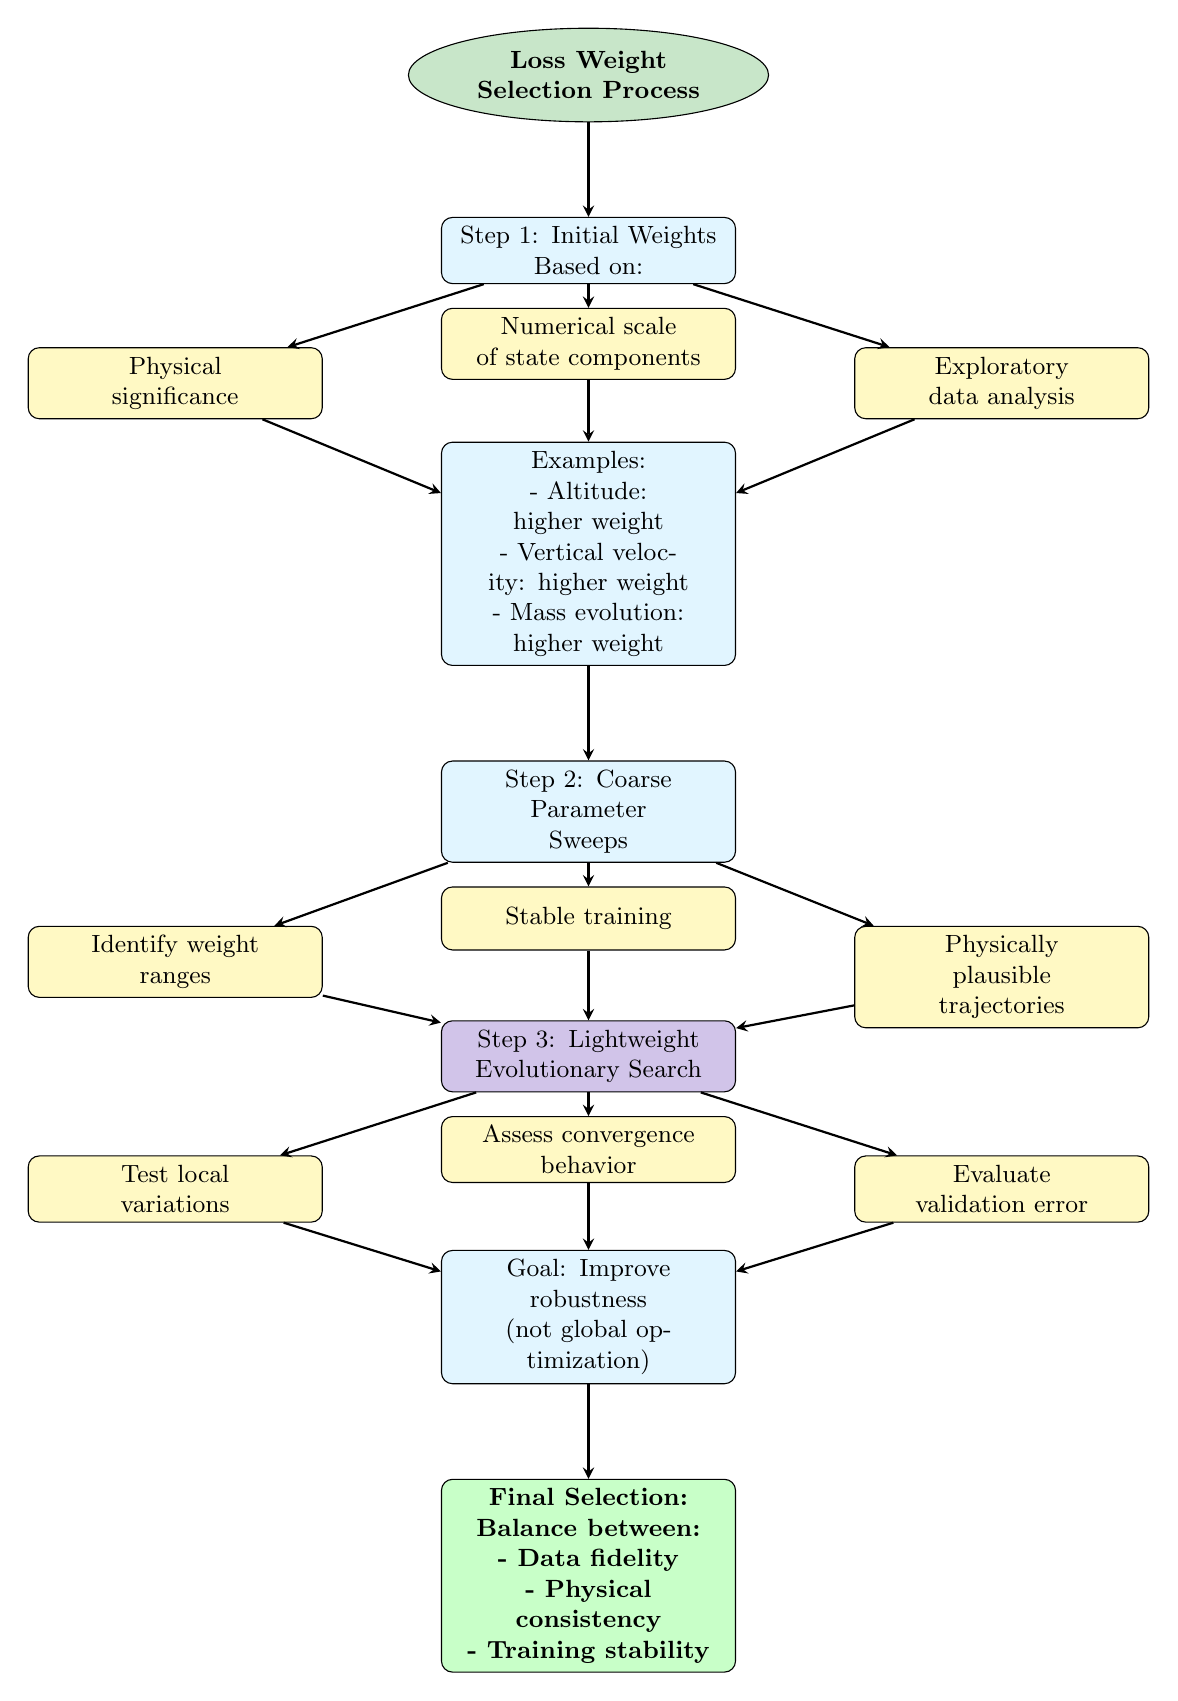
\begin{tikzpicture}[
    node distance=1.2cm and 2cm,
    every node/.style={font=\small},
    start/.style={ellipse, fill=startcolor, draw=black, text width=3cm, text centered, minimum height=0.8cm, font=\small\bfseries},
    process/.style={rectangle, rounded corners, fill=processcolor, draw=black, text width=3.5cm, text centered, minimum height=0.8cm, font=\small},
    analysis/.style={rectangle, rounded corners, fill=analysiscolor, draw=black, text width=3.5cm, text centered, minimum height=0.8cm, font=\small},
    search/.style={rectangle, rounded corners, fill=searchcolor, draw=black, text width=3.5cm, text centered, minimum height=0.8cm, font=\small},
    final/.style={rectangle, rounded corners, fill=finalcolor, draw=black, text width=3.5cm, text centered, minimum height=1cm, font=\small\bfseries},
    arrow/.style={->, >=stealth, thick, black},
    label/.style={font=\tiny}
]

% Start
\node[start] (start) {Loss Weight\\Selection Process};

% Step 1: Initial weights
\node[process, below=of start] (initial) {Step 1: Initial Weights\\Based on:};

% Initial weight factors
\node[analysis, below left=0.8cm and 1.5cm of initial] (factor1) {Physical\\significance};
\node[analysis, below=0.3cm of initial] (factor2) {Numerical scale\\of state components};
\node[analysis, below right=0.8cm and 1.5cm of initial] (factor3) {Exploratory\\data analysis};

% Examples
\node[process, below=2cm of initial] (examples) {Examples:\\- Altitude: higher weight\\- Vertical velocity: higher weight\\- Mass evolution: higher weight};

% Step 2: Parameter sweeps
\node[process, below=of examples] (sweeps) {Step 2: Coarse Parameter\\Sweeps};

% Sweep objectives
\node[analysis, below left=0.8cm and 1.5cm of sweeps] (obj1) {Identify weight\\ranges};
\node[analysis, below=0.3cm of sweeps] (obj2) {Stable training};
\node[analysis, below right=0.8cm and 1.5cm of sweeps] (obj3) {Physically\\plausible\\trajectories};

% Step 3: Evolutionary search
\node[search, below=2cm of sweeps] (evolution) {Step 3: Lightweight\\Evolutionary Search};

% Search activities
\node[analysis, below left=0.8cm and 1.5cm of evolution] (search1) {Test local\\variations};
\node[analysis, below=0.3cm of evolution] (search2) {Assess convergence\\behavior};
\node[analysis, below right=0.8cm and 1.5cm of evolution] (search3) {Evaluate\\validation error};

% Goal
\node[process, below=2cm of evolution] (goal) {Goal: Improve robustness\\(not global optimization)};

% Final selection
\node[final, below=of goal] (final) {Final Selection:\\Balance between:\\- Data fidelity\\- Physical consistency\\- Training stability};

% Arrows
\draw[arrow] (start) -- (initial);
\draw[arrow] (initial) -- (factor1);
\draw[arrow] (initial) -- (factor2);
\draw[arrow] (initial) -- (factor3);
\draw[arrow] (factor1) -- (examples);
\draw[arrow] (factor2) -- (examples);
\draw[arrow] (factor3) -- (examples);

\draw[arrow] (examples) -- (sweeps);
\draw[arrow] (sweeps) -- (obj1);
\draw[arrow] (sweeps) -- (obj2);
\draw[arrow] (sweeps) -- (obj3);
\draw[arrow] (obj1) -- (evolution);
\draw[arrow] (obj2) -- (evolution);
\draw[arrow] (obj3) -- (evolution);

\draw[arrow] (evolution) -- (search1);
\draw[arrow] (evolution) -- (search2);
\draw[arrow] (evolution) -- (search3);
\draw[arrow] (search1) -- (goal);
\draw[arrow] (search2) -- (goal);
\draw[arrow] (search3) -- (goal);

\draw[arrow] (goal) -- (final);

\end{tikzpicture}

\end{document}

